\chapter{Introduction}
\label{ch:fscf-intro}


%%%%%%%%%%%%%%%%%%%%%%%%%%%%%%%%%%%%%%%%%%%%%%%%%%%%%%%%%%%%%%%%%%%
\section{The Long-Baseline Neutrino Facility for DUNE}
\label{sec:pdr-intro-fscf}

The global neutrino physics community is developing a multi-decade physics program to measure unknown parameters of the Standard Model of particle physics and search for new phenomena. The program will be carried out as an international, leading-edge, dual-site experiment for neutrino science and proton decay studies, which is known as the \textit{Deep Underground Neutrino Experiment (DUNE)}, supported by the \textit{Long-Baseline Neutrino Facility (LBNF)}.

To achieve its ambitious physics objectives as a world-class facility, this program has been conceived around three central components: 
\begin{enumerate}
\item an intense, wide-band neutrino beam 
\item a fine-grained near neutrino detector just downstream of the neutrino source 
\item a massive liquid argon time-projection chamber (LArTPC) deployed as a far neutrino detector deep underground, 1,300 km downstream; this distance between the neutrino source and far detector -- the \textit{baseline} -- is measured along the line of travel through the Earth 
\end{enumerate}
The neutrino beam and near detector will be installed at the Fermi National Accelerator Laboratory (Fermilab), in Batavia, Illinois. The far detector will be installed at the Sanford Underground Research Facility (SURF) in Lead, South Dakota.
The experiment's detectors at the two sites will be designed, built, commissioned and operated by the international DUNE Collaboration.  LBNF is the facility designed to support the experiment. LBNF will comprise 
\begin{itemize}
\item the world's highest-intensity neutrino beam at Fermilab
\item a set of underground caverns to house the DUNE far detector modules at SURF 
\item a beamline measurement system at the near site
\item conventional facilities at both the near and far sites
\item cryogenics infrastructure to support the DUNE detector at the far site
\end{itemize}

LBNF is hosted by Fermilab and its design and construction is organized as a DOE/Fermilab project incorporating international partners. 


%%%%%%%%%%%%%%%%%%%%%%%%%%%%%%%%%%
\section{Strategy and Requirements}
\label{sec:fs-facil-cf}

The strategy for executing the scientific program was presented in the LBNF/DUNE Conceptual Design Report (CDR)\cite{cd-1-r-cdr}. The program has been developed to meet the requirements set out in the P5 report \cite{p5report2014} and takes into account the recommendations of the European Strategy for Particle Physics\cite{euro-strat-2013}. It adopts a model in which U.S. and international funding agencies share costs on the DUNE detectors, and the European Organization for Nuclear Research (CERN) and other participants provide in-kind contributions to the supporting infrastructure of LBNF. LBNF and DUNE will be tightly coordinated as DUNE collaborators design the detectors and infrastructure that will carry out the scientific program.

The requirements on LBNF derive from the DUNE Collaboration science requirements\cite{dune-sci-req}, which drive the space and functional needs of the far detector construction and operation, and from 
Environment, Safety and Health (ES\&H) and facility operations requirements. 
 The LBNF and DUNE requirements are maintained together in~\cite{dune-sci-req}.
Conventional Facility requirements are detailed in the Arup 100\% Preliminary Design Report\cite{arup:fscf100pdr}.

The DUNE far detector is designed as a set of four \ktadj{10} fiducial mass modules. 
The caverns and the services to the caverns will be as similar to one another as possible in order to implement efficiency in 
design, construction and operation. Figure~\ref{fig:underground-cavern-layout} shows the layout of the underground caverns that will house the detector modules, and the separate cavern that will house utilities and cryogenics systems. 

\begin{cdrfigure}[Underground cavern layout]{underground-cavern-layout}{Underground cavern layout (SRK, Courtesy SURF)}
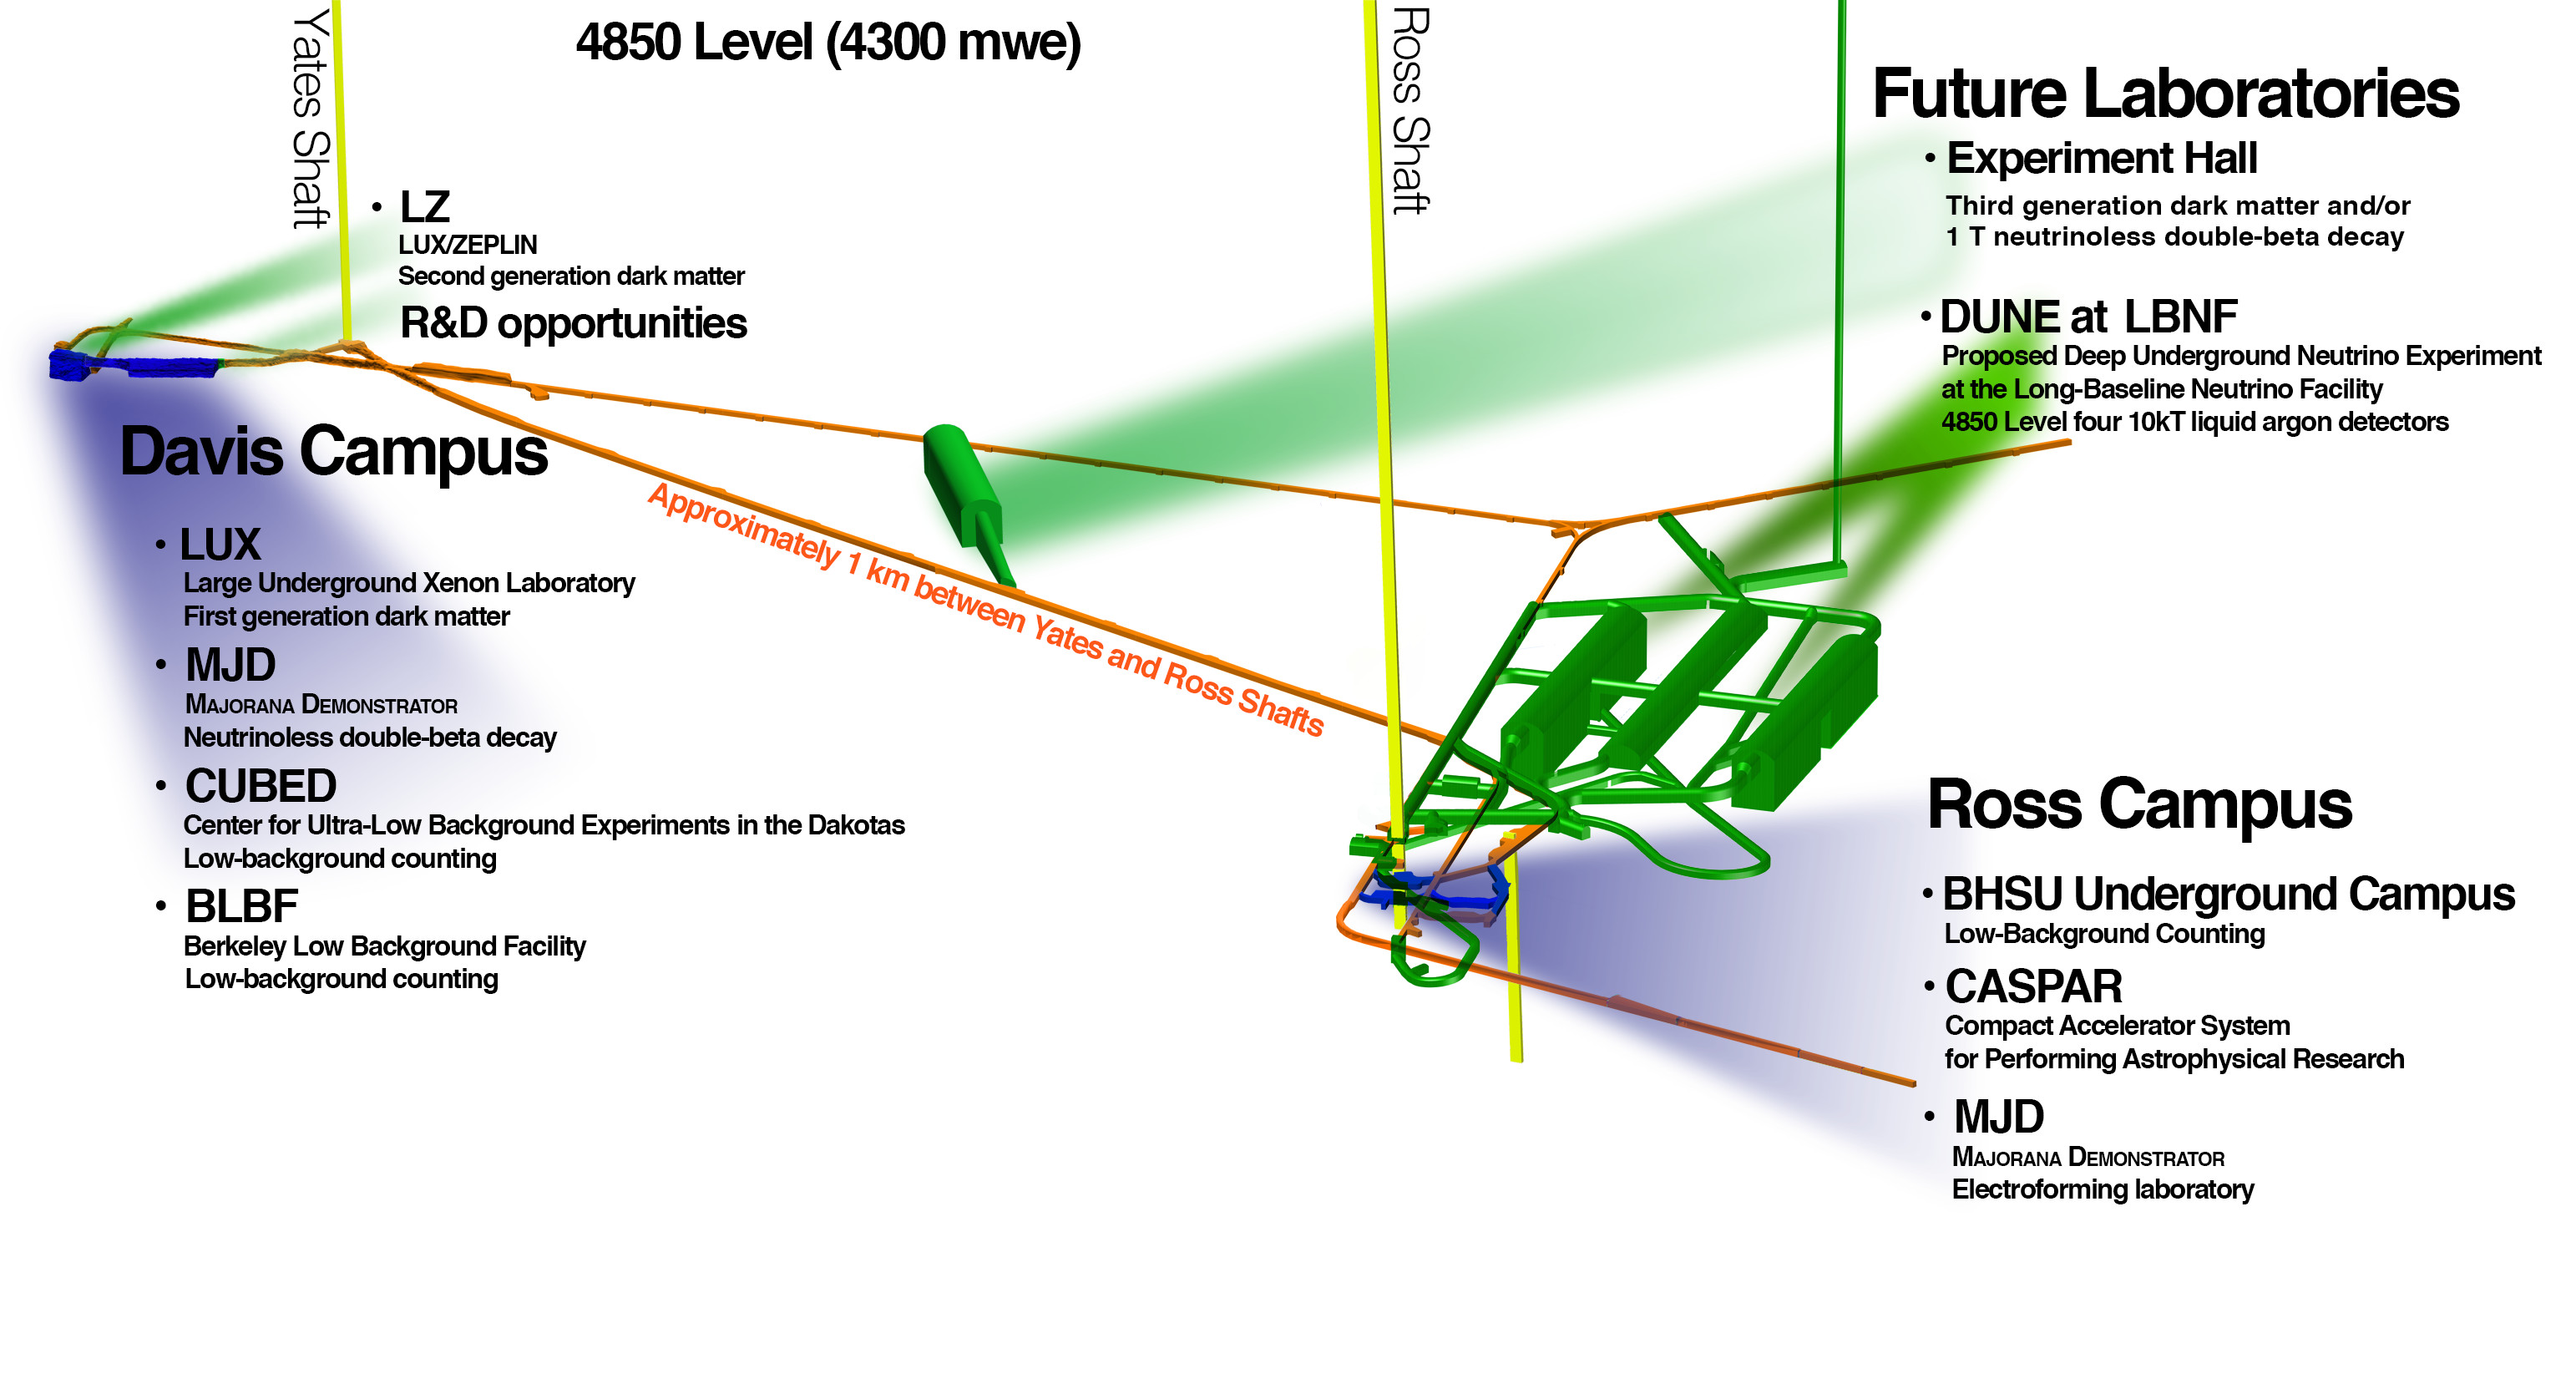
\includegraphics[width=0.8\textwidth]{underground-cavern-layout}
\end{cdrfigure}


While the SURF site already meets many of the requirements from the geological, scientific and engineering standpoints, significant work is required to provide %adequate 
the space and %the 
infrastructure %support needed 
for the experiment's installation and operation. 

This PDR presents the scope of the LBNF Far Site Conventional Facilities (FSCF) at SURF, the present and future states of the site, evaluation and assessment of its facilities and the %associated 
provisioning of associated infrastructure such as power, water, plumbing, ventilation, etc. Also described are the  %steps 
tasks and processes planned for developing the surface and underground structures and the requisite safety measures. 


%%%%%%%%%%%%%%%%%%%%%%%%%%%%%%%%%%
\section{Introduction to the Far Site Conventional Facilities}
\label{sec:fs-facil-cf}

The scope of the FSCF includes design and construction for facilities on the surface and underground at SURF for DUNE. 

The %key 
primary element of the Far Site Conventional Facilities (FSCF) is the set of underground spaces required to install, operate and support the multi-module cryogenic DUNE far detector. 
%\fixme{I moved next sentence from ch 5 to here 10/9}
The deep-underground installation is required to shield the sensitive detector from cosmic rays, as detailed in the Report on the Depth Requirements for a Massive Detector at Homestake~\cite{depth-doc}. The 4850L is deeper than what is absolutely required, but is used because of existing access at this level. 
%
The underground conventional facilities include new excavated spaces at the 4850L for the detector modules, utility spaces for experiment equipment, utility spaces for facility equipment, drifts for access, and spaces required for construction. Underground infrastructure that FSCF must provide for DUNE includes power to experiment equipment, cooling systems for that equipment and cyberinfrastructure for data collection. Underground infrastructure %necessary 
required for the facility includes domestic (potable) water, industrial water for process use and fire suppression, fire detection and alarm systems, normal and standby power systems, a sump-pump drainage system for native and leak water around the detector, water drainage to the facility-wide pump discharge system, and cyberinfrastructure for communications and security. In addition to providing new spaces and infrastructure underground, FSCF enlarges some existing spaces for use, such as the access drifts from the Ross Shaft to the new caverns, and provides infrastructure for these spaces. New piping is provided in the shaft for cryogens (gas argon transfer line and nitrogen compressor suction and discharge lines) and water as well as for power cables and cyberinfrastructure. 

About 50 buildings and utilities exist above-ground at SURF, a few of which will be utilized for LBNF. 
The scope of the surface FSCF includes only that work necessary for LBNF; it does not include the general rehabilitation of buildings on the site, which remains the responsibility of SURF. Electrical substations and distribution will be upgraded to increase power and provide standby capability for life safety. %Additional surface scope includes remodeling of 
An existing building will be remodeled to house both office space and an experiment/facility control room, and a new building will be constructed near the existing Ross Shaft to support cryogen transfer from the surface to the 4850L. To reduce the risk of failure of aging but essential support equipment during the construction and installation periods, several SURF infrastructure-reliability activities are included in the earlier phases %as early activities in 
of the LBNF Project. These include completion of the Ross Shaft rehabilitation, rebuilding of hoist motors, and replacement of the Oro Hondo fan. Failure of any of this aging infrastructure could limit or stop access to the underground.


%%%%%%%%%%%%%%%%%%%%%%%%%%%%%%%%%%%%%%%%%%%%%%%%%%%%%%%%%%%%%%%%%%%
\section{The LBNF Far Site CF Preliminary Design Report}
\label{sec:pdr-org-fscf}

The \textit{LBNF Far Site Conventional Facilities Preliminary Design Report} describes the preliminary designs for the conventional facilities planned for the Sanford Underground Research Facility (SURF), the LBNF Far Site. This document is an evolution of \textit{LBNF/DUNE CDR Annex 3C: Conventional Facilities (CF) at the Far Site}, which was prepared for the LBNF/DUNE CD-1-Refresh Review in July 2015. 
The original LBNF/DUNE Conceptual Design Report volumes have been updated~\cite{design-doc-lbnf-dune, design-doc-dune-physics, design-doc-lbnf, design-doc-dune-det}  as required to provide context for the LBNF Far Site Conventional Facilities design.


The scope of this Preliminary Design Report (PDR) is limited to the LBNF Far Site Conventional Facilities (FSCF); the cryogenics infrastructure is not included.
\begin{enumerate}
\item This chapter provides a short introduction to LBNF, DUNE and the FSCF.
\item Chapter~\ref{ch:intro-pm} summarizes the management structure for LBNF.
\item Chapter~\ref{ch:fscf-site-cond} describes the existing site conditions at SURF. 
\item Chapter~\ref{ch:fscf-surf-facil} describes the existing and planned surface buildings that will support the DUNE far detector, planned for installation at the 4850L of SURF.
\item Chapter~\ref{ch:fscf-excav} discusses the planned underground excavation. 
\item Chapter~\ref{ch:fscf-und-infra} describes the underground infrastructure necessary to facilitate installation and operation of the DUNE far detector modules.
\item Chapter~\ref{ch:fscf-siteprep} describes the restoration and maintenance activities required at the SURF site that
are included in the overall LBNF Project and planned to be executed as early Site Preparation.
\end{enumerate}

This PDR is supported by a Design Report from the independent engineering firm, Arup, USA\cite{arup:fscf100pdr}.


